Flood scenarios produced pronounced disruptions in Chennai's urban accessibility structure. The comparison of street networks under normal (NAINr3000, NACHr3000) and flood conditions (NAINr3000, NACHr3000 flood scenario) revealed a systemic reduction in accessibility. Street segments decreased by 6.56\% post-flood impact. Global accessibility indices dropped significantly: NAINr3000 by 19.74\% and NACHr3000 by 18.10\% (Figure 3). In finer-grained, local analyses (r800 radius), accessibility fell by 15.23\% for NAINr800 and by 3.14\% for NACHr800 (Figure 4). These reductions highlight the spatial fragility of Chennai's urban fabric under extreme hydrological events (Table 1).

\begin{figure}[ht]
  \centering
  \includegraphics[width=\textwidth,page=2]{../../figures/chennai_maps.pdf}
  \caption{Global and local accessibility under normal and flood conditions (source atlas: \texttt{figures/chennai\_maps.pdf}).}
\end{figure}

\begin{table}[ht]
  \centering
  \caption{Mean values of accessibility indicators and network segments under normal and flood conditions.}
  \begin{tabular}{lrrr}
    \toprule
    Metric & Normal & Flood & Difference \\
    \midrule
    Segments & -- & -- & -6.56\% \\
    NAIN r3000 & 0.8217 & 0.6595 & -19.74\% \\
    NACH r3000 & 0.8110 & 0.6642 & -18.10\% \\
    NAIN r800 & 0.9219 & 0.7815 & -15.23\% \\
    NACH r800 & 0.8458 & 0.8192 & -3.14\% \\
    \bottomrule
  \end{tabular}
\end{table}

Accessibility loss manifested heterogeneously across critical urban functions, with marked differences among urban fragments. High-risk areas accounted for a significant proportion of degraded accessibility: 35 health infrastructure units, 72 educational facilities, 163 slums, and 45 shelters were in high-risk zones. Health services and slums exhibited the highest concentration in these high-risk fragments, reflecting acute vulnerabilities during extreme flood events. Educational facilities also faced considerable exposure, with a notable number situated in zones with high penalty accessibility loss. Conversely, most shelters were distributed in fragments categorized as null or moderate risk, yet a non-negligible portion remained exposed within highrisk areas. These findings underline systemic misalignments between critical services and resilient urban structures, leaving essential infrastructure and marginalized communities especially vulnerable during flood events. The analysis of urban land use across different fragments revealed that residential areas accounted for the largest share of flood-affected zones, particularly in the highly impacted categories. Agricultural and open space areas demonstrated lower exposure, while commercial and institutional zones were moderately impacted. Fragments with a predominance of residential and mixed-residential land uses displayed the greatest decline in accessibility (Figure 5). This spatial configuration underscores the vulnerability of densely populated and economically vital areas, emphasizing the urgent need for targeted resilience strategies in these land use categories. Detailed evaluation from Table 2 shows differentiated impacts across city fragments. In Fragment 1, critical infrastructures such as health and educational services, slums, and shelters concentrated significantly in high-risk zones, with health units and slums showing the most acute vulnerability. Fragment 2 exhibited a comparatively moderate distribution, while Fragment 3, though smaller in size, demonstrated a disproportionately high exposure of slums and shelters to flood risk. Fragment 4 presented the highest number of affected slums and shelters across all categories, indicating extreme vulnerability. Fragment 5, despite its smaller representation, continued the pattern of infrastructure exposure to high-risk areas. This fragment-by-fragment breakdown highlights the heterogeneity of urban vulnerability and supports the design of localized, fragment-specific resilience interventions.

number of blocks

level of risk per fragment

Figure 5. Critical infrastructure overlaid with flood level of risk in the five- fragments. The map highlights the distribution of services (health, education, slums, shelters) in relation to spatial risk categories across Chennai's five urban fragments.

level of risk per fragment

number of infraestructure or services

Table 2. Overlay of infrastructure or services and accessibility class by urban fragment.

Global-Scale Strategies: Emergency Routes and Critical Zone Identification The top 20\% of highly accessible routes (NACHr3000 under normal conditions) served as the backbone for modelling emergency priority networks. Integrating these routes with the floodconditioned accessibility model enabled the identification of strategic corridors essential for evacuation and supply continuity. The emergency response network specifically ensured the connection of Chennai's most critical infrastructures, including the main hospitals, the airport, and the port, as well as the densest urban areas. Emergency response routes, limited to the main connections network, were proposed as a strategic guide to optimize the allocation of emergency resources during flood events. Specific interventions were tailored according to infrastructure type: for streets, strategies included gutter inclination adjustments, the elevation of evacuation pathways, and the reinforcement of Water-Sensitive Design principles; for bridges, interventions emphasized structural reinforcement, elevation to mitigate flood impacts, and ensuring redundancy in case of partial network failure. These proposals aim to enhance the functionality of the principal mobility corridors under extreme conditions (see Figure 6).

\begin{figure}[ht]
  \centering
  \includegraphics[width=\textwidth,page=6]{../../figures/chennai_maps.pdf}
  \caption{Priority corridors and city-wide intervention areas under flood conditions (source atlas: \texttt{figures/chennai\_maps.pdf}).}
\end{figure}

Leveraging a Digital Elevation Model (Copernicus GLO-30), which served to identify the city's lowest-lying areas, combined with waterways and water bodies data from the India Water 

Resources Information System, a comprehensive floodplain analysis was conducted. The identified low-lying zones were cross-referenced with high flood-risk areas, showing strong spatial coincidence. Based on this overlap, zones suitable for floodplain excavation were proposed, prioritizing large open spaces identified through recent satellite imagery. Furthermore, areas where residential buildings were detected using Google's Open Buildings dataset were flagged for density management or growth restriction strategies, aiming to mitigate future flood vulnerability through adaptive urban planning. This multi-layered model provided the foundation for a robust global-scale resilience strategy, balancing immediate flood responses with long-term urban planning interventions (see figure 7).

Figure 7. Proposed floodplain intervention zones based on elevation and hydrological data.

At a local scale (NAINr800 and NACHr800), a complementary waterways and flood-impacted street network model was developed, offering a foundation for hybrid land-water mobility strategies. Although primarily designed to evaluate accessibility during floods, this model remains available for future expansion into integrated resilience frameworks. Local-Scale Strategies: Safe Zones and Shelter Accessibility The waterways and flood street network model were utilized to assess the accessibility of existing emergency boat deployment points managed by the Greater Chennai Corporation (see figure 8). 

Analysis revealed that 30.38\% of boat locations were within highly accessible zones (NAINr800 > 1.0), while 31.65\% were positioned in areas of lowest accessibility (NAINr800 $\leq$ 0.6). A more detailed histogram breakdown showed that 8.86\% of boats were in zones of excellent accessibility (NAINr800 > 1.2), 21.52\% in high-accessibility zones (1.0 < NAINr800 $\leq$ 1.2), and 22.78\% in moderately accessible areas (0.8 < NAINr800 $\leq$ 1.0), reinforcing the uneven distribution of resources across accessibility gradients (figure 9 and table 3). This distribution highlights critical vulnerabilities, particularly for peripheral and flood-prone neighbourhoods, underscoring the need for strategic relocation or augmentation of boat deployment points. This uneven distribution of emergency boat resources suggests critical gaps in flood-time accessibility, especially in peripheral and low-lying neighbourhoods. The model highlights strategic locations where new or relocated boat points could enhance flood resilience, supporting the development of hybrid land-water evacuation networks. Although primarily serving to evaluate current operational capacities, the accessibility model also establishes a baseline for future resilience strategies, enabling Chennai to incorporate waterbased mobility into its urban adaptation planning.

Figure 8. Distribution of emergency boats under flood conditions.

The figure shows the location of deployed emergency boats in relation to floodadjusted accessibility (r800), highlighting spatial disparities in coverage across safe and vulnerable zones.

Figure 9. Accessibility histogram of emergency boat locations (NAINr800)

Measures NAINr800m

boats

(\%)

NAINr800m > 1.2

8.86\%

1.0 < NAINr800m $\leq$ 1.2

21.52\%

0.8 < NAINr800m $\leq$ 1.0

22.78\%

0.6 < NAINr800m $\leq$ 0.8

15.19\%

NAINr800m $\leq$ 0.6

31.65\%

Table 3. Distribution of emergency boat locations (NAINr800)

A k-means clustering analysis based on normalized population density, global accessibility (NAINr3000), and local accessibility (NAINr800) revealed ten distinct safe clusters within the norisk zones (see Figure 10). Clusters 7 and 9 emerged as the most strategically important safe zones. Cluster 7, while comprising only 90 blocks, displayed a highly concentrated and cohesive distribution pattern, predominantly located within specific city sectors, making it ideal for focused and immediate intervention strategies. Cluster 9, by contrast, included 50,424 blocks, with a broad geographic distribution across the city's five main urban fragments. Its dispersion allows for a widespread coverage of resilience actions, ensuring accessibility to a wider population base. Additionally, Cluster 9 exhibited consistently high normalized population density (0.43906) and accessibility (NAINr800 of 0.41081 and NAINr3000 of 0.33262), supporting its designation as a critical backbone for local-scale resilience strategies (see table 4 and 5). This detailed assessment confirms that Clusters 7 and 9 provide complementary opportunities: one for concentrated resource allocation and the other for widespread territorial resilience planning, making them priority candidates for safe zone designation and strategic emergency planning.

\begin{figure}[ht]
  \centering
  \includegraphics[width=\textwidth,page=4]{../../figures/chennai_maps.pdf}
  \caption{Population density, accessibility, and safe zones under normal and flood conditions (source atlas: \texttt{figures/chennai\_maps.pdf}).}
\end{figure}

Shelter evaluation indicated that a substantial portion of existing emergency shelters were not optimally located (see Figure 11). Detailed analysis using the Range-Shelters table revealed that only 41 shelters (22.4\% of the total) were located within the optimal 100--400-meter distance from highly accessible areas. A smaller number, 14 shelters (7.6\%), were situated within 50-100 meters, and just 8 shelters (4.4\%) were positioned within the ideal proximity of 10-50 meters. Alarmingly, 89 shelters (48.6\%) were located over 400 meters away, significantly reducing their effective accessibility during flood emergencies (see table 6). This misalignment highlights critical gaps in current emergency infrastructure planning and signals the need for a strategic reassessment of shelter locations to ensure timely and equitable access for the most vulnerable populations during extreme events.

\begin{figure}[ht]
  \centering
  \includegraphics[width=0.8\textwidth,page=5]{../../figures/chennai_maps.pdf}
  \caption{Shelter evaluation and accessibility under flood conditions (source atlas: \texttt{figures/chennai\_maps.pdf}).}
\end{figure}

Cluster

Normalized\_Population Density

0.16478

0.34052

0.23625

0.30099

0.69862

0.22445

0.49269

0.42266

0.43906

0.48422

Normalized\_NAINr800

0.29464

0.28554

0.40100

0.91973

0.26662

0.20296

0.61516

0.20180

0.41081

0.29869

Normalized\_NAINr3000

0.24595

0.25831

0.31962

0.92057

0.23364

0.18593

0.60203

0.18714

0.33262

0.26100

Table 4. Results of k-mean process with normalized values of population and NAIN identifies Zones 7 and 9 as high-priority safe zones for flood preparedness and local intervention. Number of blocks in each cluster

76956.000

128831.000

41142.000

5.000

48681.000

70231.000

90.000

93296.000

50424.000

96273.000

Cluster

Table 5. Number of blocks in each cluster

Figure. 11. Distribution of emergency shelters under flood conditions. Range >401 m 100-400 m 50-100 m 10-50 m 0-10 m

Shelters

Table 6. Shelter distribution by walking distance under flood conditions (NAINr800)

The results consolidate into a comprehensive, multi-scalar resilience framework. At the global scale, critical corridors, floodplain interventions, and emergency routes were identified to safeguard urban systems under extreme events. Locally, clustering analysis pinpointed safe zones for emergency shelter prioritization, while boat accessibility evaluations highlighted urgent areas for mobility reinforcement. This integrated approach not only addresses immediate hydrological threats but also lays the groundwork for a future-proof urban system, capable of absorbing, adapting, and responding to intensifying hydro-climatic pressures. The methodologies and findings present a replicable, scalable model for other flood-vulnerable cities navigating the complexities of urban resilience in the 21st century.
